\documentclass[../../Cours_M1.tex]{subfiles}

\title{TP1 : Introduction aux systèmes asservis échantillonés : synthèse de correcteurs analogiques numérisés}
\author{Aymeric Arnould, Tom Colinot}

\begin{document}

\maketitle

\subsection*{Effets de l'échantillonnage}

\subsubsection*{Préparation 1}
\begin{itemize}
\item Soit un signal sinusoïdal $x(t) = \sin(2 \pi f_0 t)$ échantillonné à la fréquence $F_e = 1/T_e$. Le spectre d'un signal purement sinusoïdal de fréquence $f_0$ est un Dirac de valeur 1 en $f_0$ et un Dirac de valeur -1 en $-f_0$. L'échantillonnage provoque une périodicité de ce spectre, de fréquence $F_e$.

En effet, l'échantillonnage du signal revient à le multiplier par un peigne de Dirac : 
\[p(t) = \sum_{n=0}^{\infty} \delta_0(t-nT_e) = \sum_{k=-\infty}^{\infty} \frac{1}{T_e} e^{j\frac{2\pi k t}{T_e}} \]

On peut donc exprimer le signal échantillonné $x^*(t)$ puis sa transformée de Fourier :
\begin{align*}
& x^*(t) = x(t).p(t) = \frac{1}{T_e} \sum_{k=-\infty}^{\infty}x(t)e^{-j\frac{2\pi kt}{T_e}} \\
& X^*(\omega)= \frac{1}{T_e} \sum_{k=- \infty}^{\infty}X(2\pi f-j\frac{2\pi k}{T_e}) \\
& \boxed{X^*(f)= \frac{1}{T_e} \sum_{k=- \infty}^{\infty}(\delta(f_0-kF_e) - \delta(-f_0-kF_e))} \text{ car } X(f) = \delta_{f_0}(f) - \delta_{-f_0}(f)
\end{align*}

\begin{figure}[h!]
\centering
\begin{tikzpicture}
\draw [>=latex,->] (-6,0) -- (6,0) node[right]{$f$} ;
\draw [>=latex,->] (0,-2) -- (0,2) node[left]{$|X(f)|$};
\draw [red] (1,0)node[below]{$f_0$} -- (1,1);
\draw [red] (-1,0)node[above]{$-f_0$} -- (-1,-1);
\draw (5,0)node[below]{$f_0+F_e$} -- (5,1);
\draw (3,0)node[above]{$-f_0+F_e$} -- (3,-1);
\draw (-3,0)node[below]{$f_0-F_e$} -- (-3,1);
\draw (-5,0)node[above]{$-f_0-F_e$} -- (-5,-1);
\draw [dotted] (-6,1) node[left]{$1/T_e$} -- (6,1);

\end{tikzpicture}
\caption{Représentation du spectre $X^*(f)$ dans le cas où $F_e > 2f_0$}
\end{figure}

\item Pour la reconstruction du signal, on utilise un filtre passe-bas idéal :
\[ H(p=j2\pi f) = \left\{
\begin{array}{ll}
1 & \si |f| \leq F_e/2 \\
0 & \sinon
\end{array}
\right.
\]

\begin{itemize}
\item Si $f_0 < F_e / 2$, alors on va couper toutes les composantes sauf celles en $f_0$ et en $-f_0$. Le signal reconstitué sera donc le signal sinusoïdal initial.
\item Si $f_0 = 1,2F_e$, alors le spectre sera de la forme donnée en figure 2.
\begin{figure}[h!]
\centering
\begin{tikzpicture}
\draw [>=latex,->] (-4,0) -- (5,0) node[right]{$f$} ;
\draw [>=latex,->] (0,-2) -- (0,2) node[left]{$|X(f)|$};
\draw [red] (1,0)node[below]{$f_0$} -- (1,1);
\draw [red] (-1,0)node[above]{$-f_0$} -- (-1,-1);
\draw (4.2,0)node[below]{$f_0+F_e$} -- (4.2,1);
\draw (2.2,0)node[above]{$-f_0+F_e$} -- (2.2,-1);
\draw (-0.2,0)node[below]{$f_0-F_e$} -- (-0.2,1);
\draw (-2.2,0)node[above]{$-f_0-F_e$} -- (-2.2,-1);
\draw [dotted] (-4,1) node[left]{$1/T_e$} -- (5,1);
\end{tikzpicture}
\caption{Représentation du spectre $X^*(f)$ dans le cas où $F_e = 1.2f_0$}
\end{figure}

Ainsi, en utilisant le filtre passe-bas, on ne récupérera que la composante correspondant à la fréquence $f_0-F_e$, et la reconstitution sera donc incorrecte.

\end{itemize}

\end{itemize}

\clearpage
\subsubsection*{Manipulation 1}
On réalise à l'aide de Simulink l'échantillonnage et la reconstitution d'un signal de fréquence $f_0$ avec une période d'échantillonnage $T_e=1ms$ ($F_e=1kHz$).

\begin{figure}[h!]
\centering
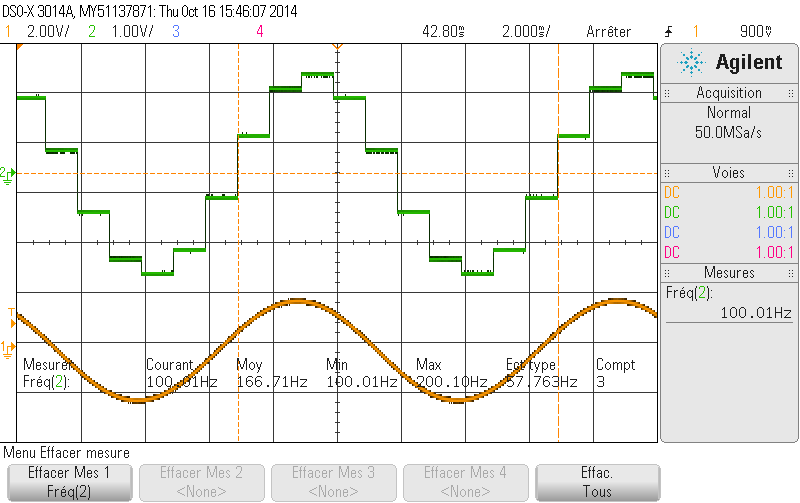
\includegraphics[scale=0.35]{m1_f0100.png}

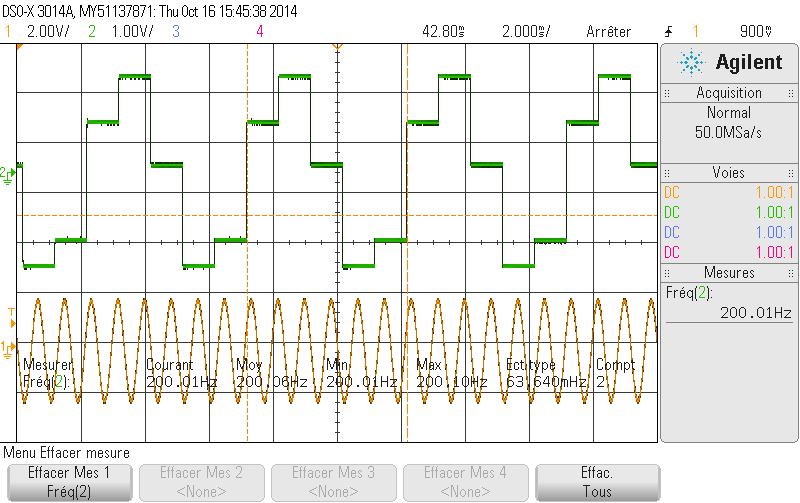
\includegraphics[scale=0.35]{m1_f01200.png}

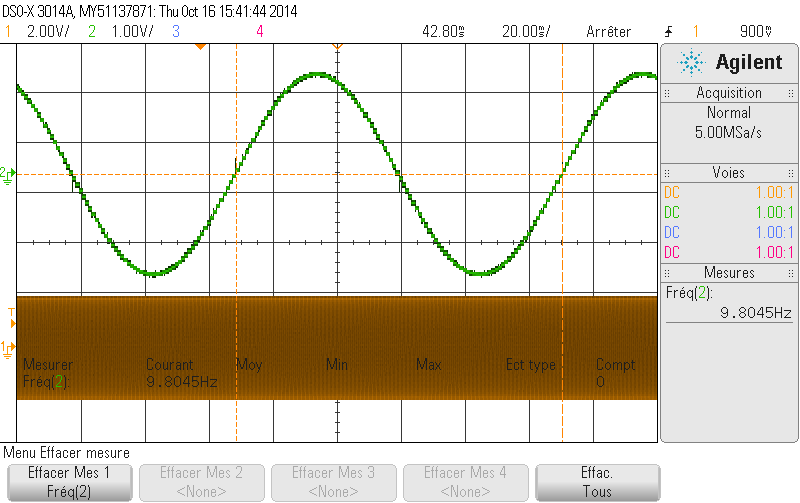
\includegraphics[scale=0.35]{m1_f04010.png}
\caption{$s(t)$ et $e(t)$ pour $f_0$ = 100Hz, 1,2kHz et 4,01kHz}
\end{figure}

\begin{itemize}
\item Lorsque $f_0 < F_e/2$, le signal est correctement reconstitué.
\item Lorsque $f_0 = 1,2F_e=1,2kHz$, comme prévu dans la préparation, on ne récupère qu'un signal avec une fréquence $f_0-F_e = 200Hz$.
\item Lorsque $f_0 \approx kF_e$ (ici $k=4$), alors on récupère de même un signal à la fréquence $f_0-kF_e$ (ici 4010-4000 = 10 Hz): c'est ce qu'on appelle un phénomène de battement.
\end{itemize}

\subsubsection*{Préparation 2}
Le système comporte dans la chaîne directe le système analogique de fonction de transfert $H(p) = \frac{1}{1+2m_{BO}\frac{p}{\omega_{0BO}}+\frac{p^2}{\omega_{0BO}^2}}$ et un correcteur $C(p) = K_p$.
\begin{itemize}
\item L'expression de la fonction de transfert en boucle fermée s'écrit donc :
\begin{align*}
H_{BF}(p) & = \frac{H(p)C(p)}{1+H(p)C(p)} \\
& = \frac{K_p}{(1+2m_{BO}\frac{p}{\omega_{0BO}}+\frac{p^2}{\omega_{0BO}^2}) + K_p} \\
H_{BF}(p) & = \frac{\frac{K_p}{K_p+1}}{1+2\frac{m_{BO}}{K_p+1}\frac{p}{\omega_{0BO}}+\frac{p^2}{(K_p+1)\omega_{0BO}^2}}
\end{align*}
\item Avec $K_p=20$, on a alors
\begin{align*}
H_{BF}(p) & = \frac{0.95}{1+3,81.10^{-4}p+3,04.10^{-6}p^2}
\intertext{On a donc :}
\frac{1}{\omega_{0BF}^2} & = 3,04.10^{-6} \et 
\frac{2m_{BF}}{\omega_{0BF}} = 3,81.10^{-4}
\intertext{On en déduit les paramètres en boucle fermée :}
\omega_{0BF} & = 574 rad.s^{-1} \\
m_{BF} & = 0,11 
\end{align*}

À l'aide de l'abaque donnant le temps de réponse réduit $t_r\omega_0$ en fonction de l'amortissement $m$, on en déduit $t_r\omega_0 = 30$ rad donc \[t_r = 52,3ms\]

L'abaque des dépassements indiciels permet d'obtenir la valeur du premier dépassement 
\[D_1 = 0.7\]

\item Le diagramme de Bode est donné en annexe 1. On assure une marge de phase de $45^o$ si on a pour une pulsation donnée une phase de $-135^o$ et un gain nul. Pour le système non corrigé, on a un gain de $-7,16dB$ pour une phase de $-135^o$. Multiplier par un gain $K_{45}=10^{7,16/20}=2,28$ permet de translater la courbe de gain sans agir sur la phase, et on a alors bien la marge de phase voulue.
\end{itemize}

\clearpage
\subsubsection*{Manipulation 2}
\paragraph{Simulation sur Simulink} On réalise l'asservissement analogique et on prend la réponse indicielle. 

Pour $K_p = 20$ on obtient la réponse indicielle donnée en annexe 5. La valeur finale est de 0.95, l'amplitude du premier dépassement est de 1.6. On a donc $D_1=\frac{1.6-0.95}{0.95}=0.68$. Le temps de réponse à $5\%$ est d'environ $50ms$.

Pour $K_p = K_{45} = 2,28$, on se propose de relever le gain et la phase à $\omega=202rad/s$ (voir annexe 6).On a bien un gain unitaire et une phase de $-135^o$ donc le gain $K_{45}$ assure bien une marge de phase de $45^o$.

\paragraph{Montage sur la maquette}
On réalise le montage sur la maquette. 

Pour $K_p=20=R_1/R_2$, on utilise $R_1=12K\Omega$ et $R_2=600\Omega$ en mettant deux résistances de $1,2k\Omega$ en parallèle.
On obtient la réponse indicielle suivante :
\begin{figure}[h!]
\centering
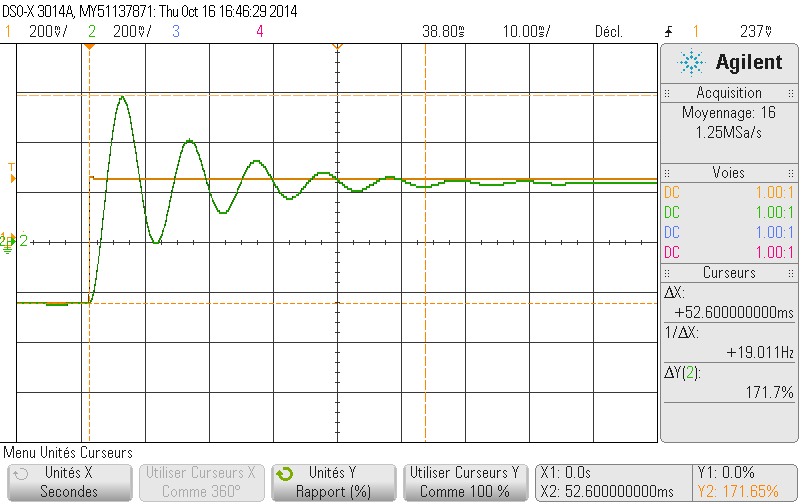
\includegraphics[scale=0.5]{m2Kp20.png}
\caption{Réponse indicielle, $K_p=20$}
\end{figure}

Les curseurs nous permettent d'avoir un temps de réponse à $5\%$ de $52ms$ et un premier dépassement de $70\%$.

\clearpage

Pour $K_p=K_{45}$, on obtient la réponse suivante à $\omega = 202rad/s$ ($f=32.2Hz$) :

\begin{figure}[h!]
\centering
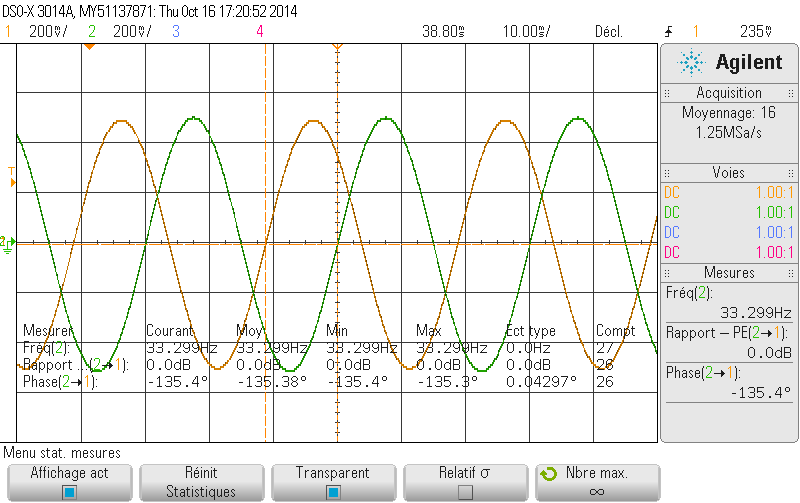
\includegraphics[scale=0.5]{m2K45w0dB.png}
\caption{$s(t)$ et $e(t)$ en boucle ouverte, $K=K_{45}$, $\omega = 202rad/s$}
\end{figure}

On a bien un gain unitaire et un déphasage de $-135^o$, donc le gain $K_{45}$ assure bien une marge de phase de $45^o$.

\bigskip

\paragraph{Conclusion partie 2} Les résultats donnés par la simulation sont conformes à ceux obtenus par expérimentation sur la plaquette. La simulation Simulink représente bien le système réel implanté sur la plaquette.

\clearpage

\subsection*{Correcteur analogique numérisé}
\subsubsection*{Préparation 3}
On modélise l'action de l'échantillonneur-bloqueur par un retard pur de fonction de transfert \[B(p) = \exp(-T_ep/2)\]

Ainsi, le gain de la fonction de transfert en boucle ouverte n'est pas affecté car $|\exp(-T_ep/2)| = 1$, et la phase est modifiée de $arg(\exp(-T_ep/2)) = -T_e/2 \omega$.

\begin{figure}[h!]
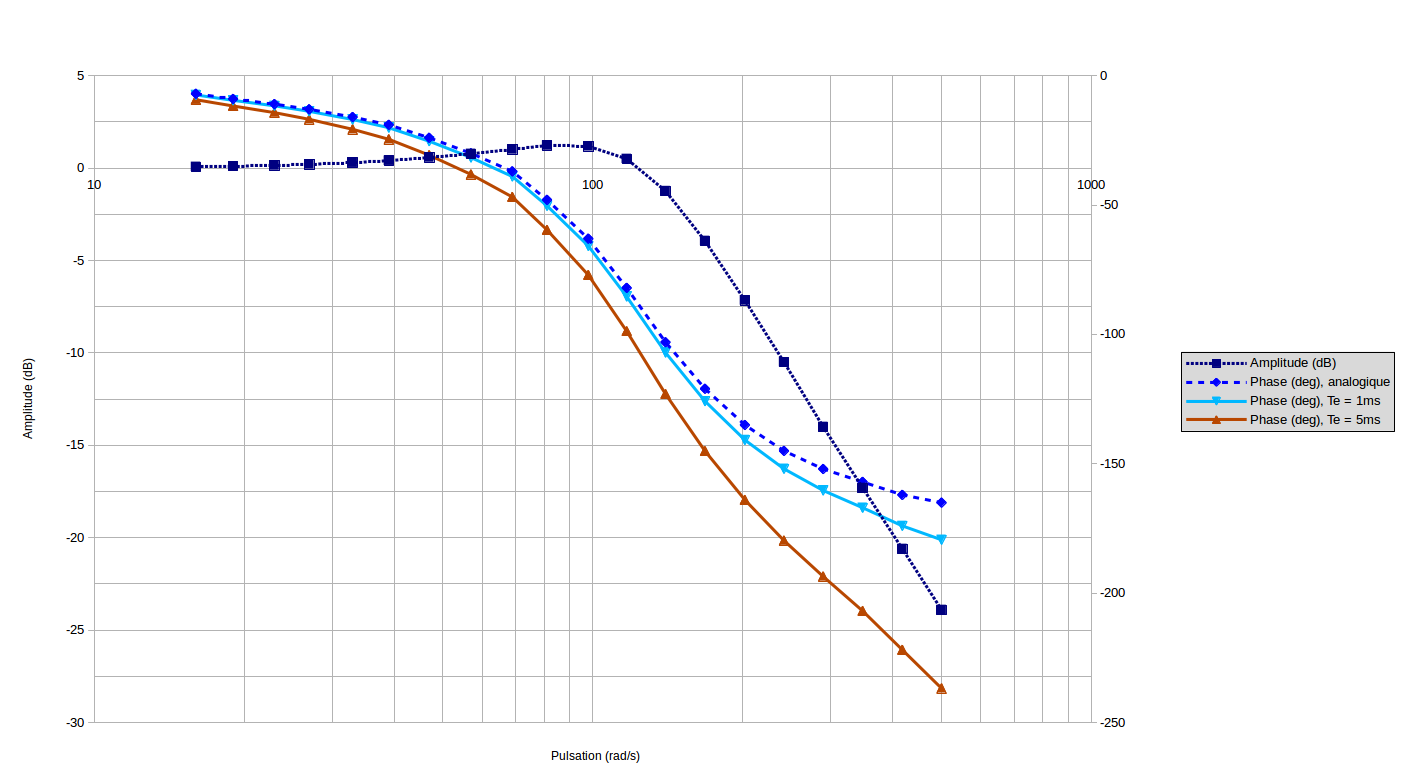
\includegraphics[scale=0.4]{Bode2.png}
\caption{Diagrammes de Bode du système analogique et échantillonné}
\end{figure}

\begin{itemize}
\item 1er cas : $T_e = 1ms$ (voir annexe 2)\\

Le gain correspondant à la phase $-135^o$ est de $-5.7dB$ pour $\omega=190rad/s$, donc on a $K_{45} = 10^{5.7/20} = 1.93$.

La limite d'instabilité est atteinte lorsqu'on a simultanément une phase de $-180^o$ et un gain de $0dB$. On a ici un gain de $-23.9dB$ pour une phase de $-180^o$, donc on a à la limite d'instabilité $K_{lim}=10^{23.9/20}=15.7$.


\clearpage

\item 2ème cas : $T_e = 5ms$ (voir annexe 3)\\

Le gain correspondant à la phase $-135^o$ est de $-2.5dB$ pour $\omega=150rad/s$, donc on a $K_{45} = 10^{2.5/20} = 1.33$.

La limite d'instabilité est atteinte lorsqu'on a simultanément une phase de $-180^o$ et un gain de $0dB$. On a ici un gain de $-10,5dB$ pour une phase de $-180^o$, donc on a à la limite d'instabilité $K_{lim}=3,35$.

\end{itemize}

\clearpage

\subsubsection*{Manipulation 3}

On se propose dans les deux cas ($T_e=1ms$, $T_e=5ms$) de vérifier que le gain $K_{45}$ assure la marge de phase à $45^o$ et que le gain $K_{lim}$ est bien la limite de stabilité.

\bigskip
\textbf{1er cas :} $T_e = 1ms$

\begin{figure}[h!]
\centering
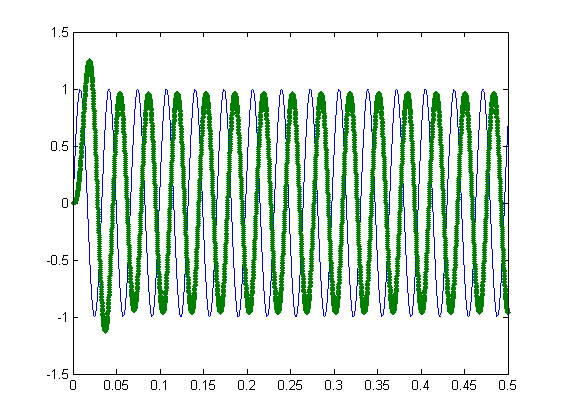
\includegraphics[scale=0.8]{m3retardpurTe1Kp45.png}
\caption{$e(t)$ et $s(t)$ en boucle ouverte, $K_p=K_{45}$, $\omega=190rad/s$}
\end{figure}

Le gain $K_{45}$ assure bien une marge de phase de $-135^o$.

\begin{figure}[h!]
\centering
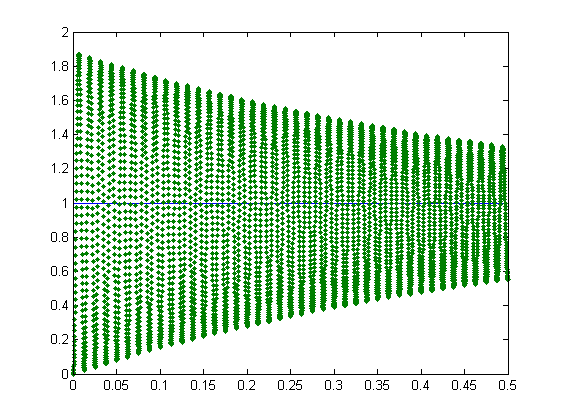
\includegraphics[scale=0.8]{m3retardpurTe1.png}
\caption{Réponse indicielle, $K=K_{lim}$}
\end{figure}

Le gain $K_{lim}$ assure bien la limite d'instabilité.

On se propose de comparer la simulation du système avec le correcteur numérique et avec sa modélisation par un retard pur.

\begin{figure}[h!]
\centering
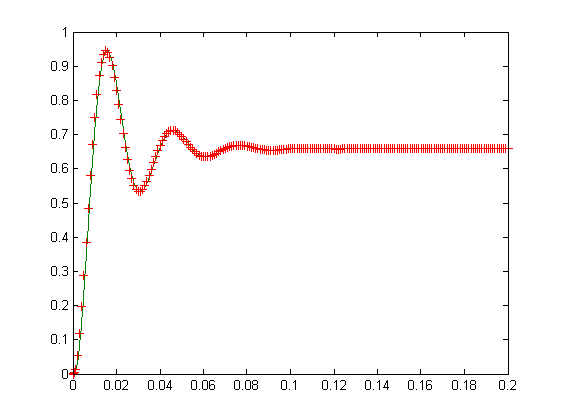
\includegraphics[scale=0.8]{m3compTe1.png}
\caption{Réponse indicielle simulée pour $K=K_{45}$, avec correcteur numérique (--) et modélisation par un retard pur (+)}
\end{figure}

La modélisation par un retard pur est très proche du comportement réel du correcteur.

En faisant le montage avec la plaquette analogique et le correcteur numérique, on retrouve une réponse semblable.

\begin{figure}[h!]
\centering
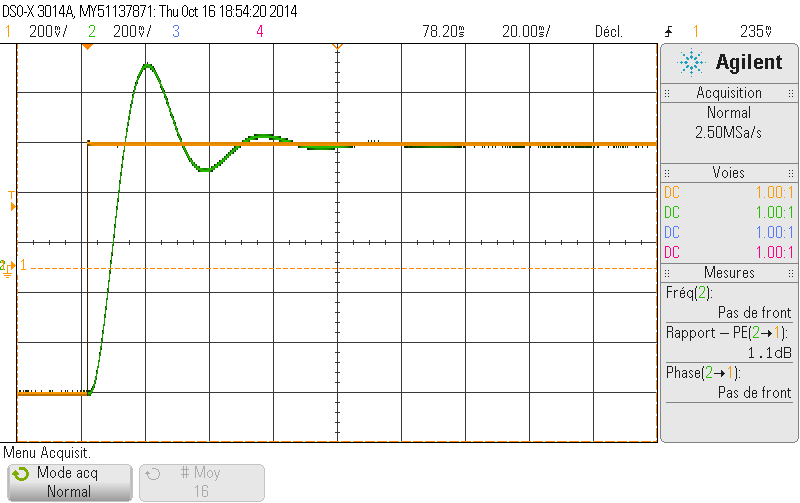
\includegraphics[scale=0.5]{m3maquette.png}
\caption{Réponse indicielle avec la maquette et le correcteur numérique pour $K=K_{45}$}
\end{figure}

\clearpage
\textbf{2ème cas :} $T_e = 5ms$

\begin{figure}[h!]
\centering
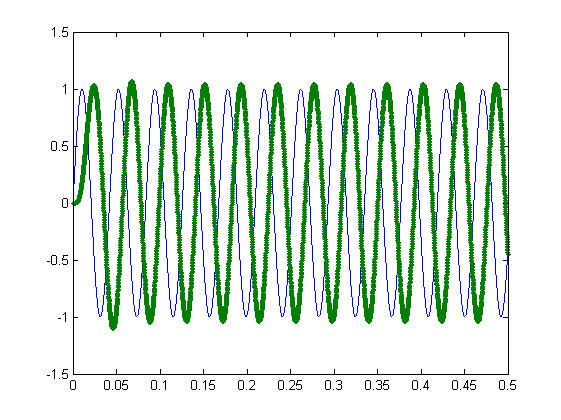
\includegraphics[scale=0.8]{m3retardpurTe5Kp45.png}
\caption{$e(t)$ et $s(t)$ en boucle ouverte, $K_p=K_{45}$, $\omega=150rad/s$}
\end{figure}

Le gain $K_{45}$ assure bien une marge de phase de $-135^o$.

\begin{figure}[h!]
\centering
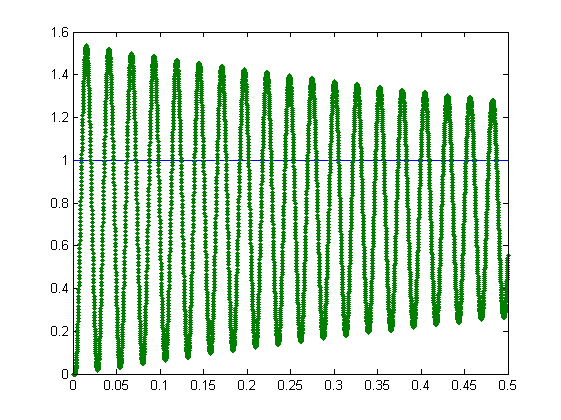
\includegraphics[scale=0.8]{m3retardpurTe5.png}
\caption{Réponse indicielle, $K=K_{lim}$}
\end{figure}

Le gain $K_{lim}$ assure bien la limite d'instabilité.

\clearpage
\subsection*{Synthèse d'un correcteur PI numérisé}
\subsubsection*{Préparation 4}

Le diagramme de Bode asymptotique du correcteur $C(p) = K_p(1+\frac{1}{T_ip})$ est le suivant :

\begin{figure}[h!]
\centering
\begin{tikzpicture}
\draw [>=latex,->] (0,0) -- (0,3) node[left]{$\phi(^o)$} ;
\draw [>=latex,->] (-1,2) -- (6,2) node[right]{$\omega$};

\draw [red] (0,1) node[left]{$-90$} -- (3,1) -- (3,2) -- (6,2);

\draw [>=latex,->] (0,4) -- (0,7) node[left]{$G_{dB}$} ;
\draw [>=latex,->] (-1,5) -- (6,5) node[right]{$\omega$};

\draw [red] (0,6.5) -- (3,5.5) -- (6,5.5);
\draw [red,dashed] (0,5.5) node[left]{$K_p$} -- (3,5.5) -- (3,2) node[left]{$\frac{1}{T_i}$};

\end{tikzpicture}
\end{figure}

Pour obtenir une marge de phase de $-45^o$, il faut utiliser $K_p$ pour ajuster la courbe de gain. Pour cela, on se place dans le domaine où le gain du correcteur est égal à $K_p$ et où la phase est nulle. 

Le gain $K_p$ utilisé sera celui calculé précédemment, $K_{45} = 2.28$.
On avait pour le système non corrigé une phase de $-135dB$ pour une pulsation de 202 rad/s. On va donc placer $\frac{1}{T_i}=\frac{202}{10}$ donc $T_i=49.5ms$.

\end{document}
